 
\chapter{Branch Prediction}

This chapter discusses how BOOM predicts and resolves branch predictions.

BOOM uses two levels of branch prediction- a single-cycle ``next-line predictor", and a slower but more complex ``backing predictor".\footnote{\TODO{Author: I'm open to better names!}}


\begin{figure}[ht]
	\centering
	\centerline{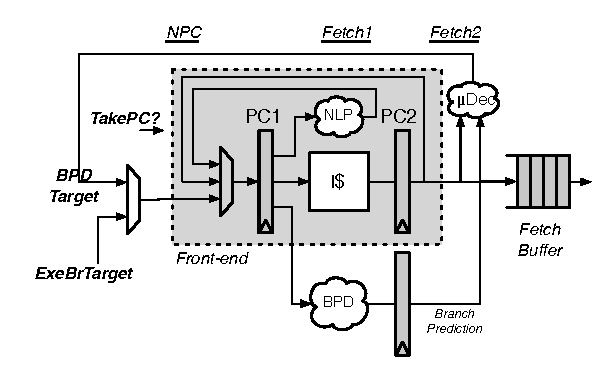
\includegraphics[scale =1] {figures/frontend}}
	\caption{ \small The Fetch Unit.}
	\label{fig:lsu}
\end{figure}


\section{The Rocket Next-line Predictor (NLP)}

BOOM instantiates the Rocket core's Front-End, which fetches instructions and predicts every cycle where to fetch the next instructions. If a misprediction is detected in BOOM's backend, or BOOM's own predictor wants to redirect the pipeline in a different direction, a request is sent to the Front-End and it begins fetching along a new instruction path. 

The next-line predictor (NLP) takes in the current PC being used to fetch instructions (the {\em Fetch PC}) and predicts combinationally where the next instructions should be fetched for the next cycle. If predicted correctly, there are no pipeline bubbles. 

The next-line predictor is an amalgamation of a fully-associative branch target buffer (BTB), a gshare branch history table (BHT), and a return address stack (RAS).  

\subsection{NLP Predictions}

The {\em Fetch PC} first performs a tag match to find a uniquely matching BTB entry.  If a hit occurs, the BTB entry will make a prediction in concert with the BHT and RAS as to whether there is a branch, jump, or return found in the {\em fetch packet} and which instruction in the {\em fetch packet} is to blame.  The BTB entry also contains a predicted PC target, which is used as the {\em Fetch PC} on the next cycle.  



The hysteresis bits (governed by a gshare predictor) are only used on a BTB entry hit and if the predicting instruction is a branch. 

If the BTB entry contains a {\em return} instruction, the RAS stack is used to provide the predicted return PC as the next {\em Fetch PC}. The actual RAS management is governed externally. 

For area-efficiency, the high-order bits of the PC tags and PC targets are stored in a compressed file.


\subsection{NLP Updates}

Each branch passed down the pipeline remembers not only its own PC, but the {\em Fetch PC} used to fetch it.\footnote{In reality, only the very lowest bits must be saved, as the higher-order bits will be the same.}  Upon Branch Resolution, the NLP is updated with the outcome of the branch.  

However, the branch's PC is not used for the BTB tag match, but rather the branch's {\em Fetch PC}.  Even for superscalar fetching, only a single {\em Fetch PC} is passed to the NLP. The NLP must predict across the entire {\em fetch packet} which of the many possible branches will be the dominating branch that redirects the PC. 


\section{The Backing Predictor}

\TODO{...}

\section{Branch Prediction Configurations}

There are a number of parameters provided to govern the branch prediction in BOOM.

\TODO{...}
 
